\section{De l'algèbre aux composants}\label{sec:contrib:astronef:preparation}
À tout composant est attachée une fabrique permettant de créer les instances. Pour construire une requête, l'utilisateur peut faire appel à chaque fabrique pour instancier chaque source, opérateur, entité, et puits. Une fois les composants construits et liés entre eux, il peut demander au moteur de créer un service \textit{QueryRuntime} pour exécuter la requête. Toutefois, nous souhaitons pouvoir exploiter les connaissances d'Astral pour aider à la construction de ce plan d'exécution.

Nous souhaitons que l'utilisateur n'ait pas à intervenir lors de cette construction. De son point de vue, il ne doit écrire que l'expression algébrique de sa requête et il doit être garanti d'une mise en œuvre efficace. Cette section détaille notre approche. Tout d'abord, nous détaillons l'idée de la construction du plan d'exécution par règles. Ensuite, nous présentons les choix technologiques mis en œuvres. Enfin, nous voyons comment préparer la requête à l'optimisation que nous détaillons dans les sections suivantes.

\subsection{Approche de la construction par inférence}
Pour atteindre ce but, nous avons choisi de mettre en place une approche à base de règle. En partant de l'expression algébrique, nous itérons suivant plusieurs règles d'inférence jusqu'à l'obtention d'un plan de requête. Nous remarquons plusieurs avantages à une telle approche :
\begin{itemize}
	\item Intégration naturelle des connaissances. Les propriétés de l'algèbre peuvent s'exprimer dans un langage déclaratif pour les exploiter.
	\item Expression de la sémantique des composants par l'algèbre. Comme il est nécessaire d'associer la sémantique d'Astral aux composants logiciels, il est nécessaire de spécifier à quelle opération chaque composant (et chaque paramètre de configuration) répond. Cela permet une clarification des sémantiques d'exécution.
	\item Extensibilité très forte. En considérant que l'ajout de nouveaux composants peut se faire via l'ajout de nouvelles règles, il devient aisé d'étendre le système pour permettre des opérateurs, ou des optimisations qui n'étaient pas prévues.
\end{itemize}

\subsubsection{Optimisation par heuristiques}
Afin de mettre en œuvre cet ensemble de règles pour obtenir un plan de requête efficace, nous introduisons une optimisation logique et physique à l'image des optimisations des SGBD. Nous restructurons la structure de l'expression algébrique dans la section~\ref{sec:contrib:astronef:logique} pour qu'elle soit plus optimisée. Ensuite, nous sélectionnons les meilleurs composants et les meilleures configurations pour mettre en œuvre cette nouvelle expression, dans la section~\ref{sec:contrib:astronef:physique}.

Toutefois, dans notre contexte, nous ne pouvons pas appliquer directement certaines optimisations des SGBDs. Contrairement aux règles habituelles, nous ne réordonnons pas les jointures du fait du théorème~\ref{thm:asymetrie}. De plus, la notion d'entrée-sortie est réduite à une notion de résultats intermédiaires, même au niveau des sources (rendant l'utilisation des index moins pertinents que sur disque). En effet, la performance se mesure généralement en débit supporté et les débits de sources sont a priori inconnus. Au total, un gain de performance est mesuré sur un gain de consommation processeur et, à moindre mesure, sur une consommation mémoire contrôlée (ou bornée).

De plus, Astral possède plus d'opérateurs et de restrictions que l'algèbre relationnelle ce qui rend l'espace de recherche plus large. Ainsi, nous développons plusieurs heuristiques nous permettant de faire les différentes réécritures par applications de règles.

\begin{figure}[ht]
	\centering
	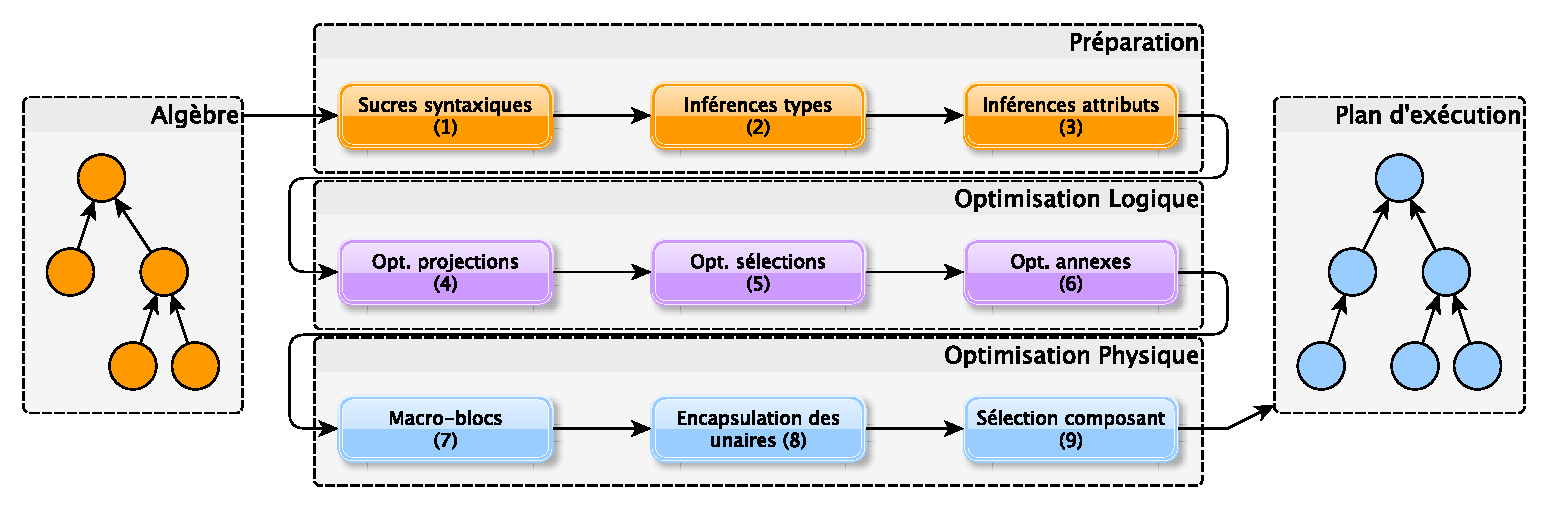
\includegraphics[width=0.9\textwidth]{contrib-astronef-optimisation}
	\caption{Processus d'optimisation d'une requête algébrique dans Astronef}\label{fig:contrib:astronef:optimisation}
\end{figure}
La figure~\ref{fig:contrib:astronef:optimisation} représente le processus total d'optimisation d'une requête algébrique. Nous pouvons clairement distinguer trois parties, la phase de préparation, puis l'optimisation logique et enfin physique. Chaque sous-tâche est détaillée dans les sections suivantes.

\subsection{Choix technologiques}
Nous utilisons un moteur capable d'exécuter du Prolog~\footnote{En réalité, le langage utilisé (PROVA~\cite{Kozlenkov:prova}) est un dérivé de Prolog mieux adapté à l'intégration avec Java. Mais le principe reste similaire.}, langage de programmation logique, pour appliquer nos règles. Avant de détailler l'ensemble de ces règles, nous présentons d'abord la structure d'une expression. Toute expression est structurée sous forme d'arbre, il est possible de représenter une requête avec des nœuds de la forme\footnote{L'utilisation d'objets de propriétés fait partie du langage PROVA, mais cela reste formalisable en Prolog standard avec une liste d'éléments [clé,valeur].} :
\begin{center} [$\underbrace{A}_{\textrm{Nature du nœud}}$, $\underbrace{B}_{\textrm{Ensemble de propriétés}}$, $\underbrace{C}_{\textrm{Liste de nœuds fils}}$] \end{center}
\begin{example}
	Soit $R$ une source déclarée dans le système, nous souhaitons exécuter la requête $\sigma_{id=1} R$. L'expression de cette requête en PROVA est la suivante :
	\begin{lstlisting}
[sigma,	{"condition":"id=1"}, [
	[source, {id:"R"}, []]
]]
	\end{lstlisting}
\end{example}
Nous remarquons que cette syntaxe est très similaire au \textit{XML} : chaque nœud possède un nom, un ensemble de propriétés et un ensemble de fils, tout comme les balises \textit{XML}. C'est pour cela que ce langage est celui utilisé en pratique pour spécifier des requêtes dans le prototype. Il est ensuite traduit en expression utilisable en Prolog. L'ensemble des nœuds possibles correspond aux différents opérateurs de l'algèbre. Nous ne détaillons pas cet aspect dans ce manuscrit. Le lecteur peut consulter le manuel sur la page web suivante \url{http://code.google.com/p/astral/wiki/XMLSyntax} pour trouver les expressions exactes supportées.

\subsection{Préparation de la requête}
Afin de pouvoir commencer à raisonner sur l'expression algébrique, nous devons tout d'abord préparer l'arbre de requête. Nous présentons l'ensemble de la phase de préparation composé du remplacement des sucres syntaxiques, de l'inférence des types et de l'inférences des attributs des résultats intermédiaires.
\subsubsection{Sucres syntaxiques}
Un sucre syntaxique permet d'aider l'utilisateur à écrire et lire son expression algébrique. Afin de pouvoir appliquer des règles sur l'arbre de requête, nous devons remplacer ces sucres syntaxiques par leurs expressions en termes d'opérateurs primitifs Astral. Par exemple, l'opérateur $\ssjoin$ est une composition d'opérateur $\Join$ et $\D_f^c$, l'opérateur $[L]$ correspond à l'opérateur $[j,j,1]$.

\begin{regle}[Sucres syntaxiques]
Le remplacement des sucres syntaxiques transformant l'expression $[A1,B1,C1]$ en $[A2,B2,C2]$ se fait par le prédicat :
\begin{center} \textbf{sugar}($[A1,B1,C1]$, $[A2,B2,C2]$).\end{center}
Ce prédicat est appliqué tant qu'il peut l'être (de manière itérative).
\end{regle}

\begin{example}
	Nous nous proposons de remplacer le sucre syntaxique $R^{t_0}$ en $\D^{t0} (R)$. $R^{t_0}$ est exprimé par le nœud \textit{freeze} possédant le paramètre \enquote{at} et $\D$ est exprimé par un nœud \textit{timetransform} possédant un paramètre \enquote{description}. Voici l'expression de ce remplacement :
	\begin{lstlisting}
sugar(
	[freeze, % Lorsqu'il existe un noeud freeze
		{at: t0},
		Children], 
	[timetransform, % ... le remplacer par timetransform
		{"description": [ % Avec un parametre description
		% contenant le type de manipulation voulue
			{"type": "freeze", 
			"at": t0}
		]},
		Children]
).
	\end{lstlisting}
\end{example}

Ce prédicat est de plus utilisé pour analyser les chaînes de caractères ce qui permet, par exemple, d'extraire la liste des attributs de conditions ou d'expressions.

\subsubsection{Inférences des types et attributs}
Afin de pouvoir traiter correctement les différents nœuds, il nous faut inférer les deux propriétés majeures de chaque nœud d'une requête qui va définir la nature de son résultat intermédiaire : son type (\textit{flux} ou \textit{relation}) et ses attributs. Pour cela, il faut être garanti que les sources exposent leurs attributs et types dans leurs propriétés. Par la suite, un programme applique ces règles de façon récursive. Les résultats sont stockés dans les propriétés \textit{type} et \textit{attributes}.

\begin{regle}[Inférences des types]
L'inférence du type $Type$ de l'expression $[A,B,C]$ dont les types fils sont $TypesFils=[T1,...]$ se fait par le prédicat :
\begin{center} \textbf{typerules}($[A,B,C,TypesFils]$, $Type$).\end{center}
Ce prédicat s'applique de manière récursive.
\end{regle}

\begin{regle}[Inférences des attributs]
L'inférence de la liste d'attributs d'un nœud $[A,B,C]$ dont les attributs fils sont $AttributsFils$ se fait par le prédicat :
\begin{center} \textbf{attribrules}($[A,B,C,AttributsFils]$, $Attributs$).\end{center}
Ce prédicat s'applique de manière récursive.
\end{regle}

\begin{example}
	Pour la définition de la jointure dans Astronef, les règles sont simples. La liste des attributs est l'union des listes d'attributs fils. Et le type de la jointure est relationnel si ses fils le sont aussi.
	\begin{lstlisting}
typerules([join,_,_, TypesFils], Type):- 
	allequal(TypesFils,Type), % Verification que tous soient relationnels 
	relation(Type), !.
attribrules([join,_,_,AttributsFils], Attributs):- !, 
	union(AttributsFils,Attributs).
	\end{lstlisting}
\end{example}

Voyons désormais un exemple simple sur la jointure de deux relations.
\begin{example}
	Soit la requête $S[B] \Join_{a < b} R$. Son expression correspondante en Prolog est :
	\begin{lstlisting}
[join, {condition: "a < b"}, [
	[window, {description: [{type: "B"}]}, [
		[source, {id: "S", attributes: ["a", "T"], type: "stream"}, []]
	]],
	[source, {id: "R", attributes=["b", "c", "d"], type: "relation"}, []]
]]
	\end{lstlisting}
	Après la phase de préparation, nous obtenons l'expression suivante :
	\begin{lstlisting}
[join, {condition: "a < b", conditionAttributes: ["a", "b"], 
		 type: "relation", attributes: ["a", "b", "c", "d", "T"]}, [
	[window, {description: [{type: "B"}], 
			   type: "relation", attributes: ["a", "T"]}, [
		[source, {id: "S", attributes: ["a", "T"], type: "stream"}, []]
	]],
	[source, {id: "R", attributes=["b", "c", "d"], type: "relation"}, []]
]]
	\end{lstlisting}
	Nous remarquons que les propriétés \textit{type} et \textit{attributes} existent sur tous les nœuds maintenant. De plus, la propriété \textit{conditionAttributes} a été placée sur la jointure.
\end{example}
Après le remplacement des sucres syntaxiques et l'inférence des types et attributs, l'évaluation procède à l'optimisation logique.
